% =============================================================================
%  A Radix-4 Booth Multiplier in Structural VHDL -- slides
%  Build:  pdflatex presentation.tex   (run twice)
% =============================================================================
\documentclass[aspectratio=169,11pt]{beamer}

\usetheme{default}
\usecolortheme{default}
\setbeamertemplate{navigation symbols}{}
\setbeamertemplate{footline}[frame number]

\usepackage[T1]{fontenc}
\usepackage[utf8]{inputenc}
\usepackage{lmodern}
\usepackage{amsmath,amssymb}
\usepackage{booktabs}
\usepackage{graphicx}
\usepackage{xcolor}
\usepackage{listings}

\definecolor{accent}{HTML}{185FA5}
\definecolor{soft}{HTML}{5F5E5A}
\definecolor{codebg}{HTML}{F7F6F2}
\definecolor{rule}{HTML}{B4B2A9}
\definecolor{good}{HTML}{0F6E56}

\setbeamercolor{frametitle}{fg=accent}
\setbeamercolor{title}{fg=accent}
\setbeamercolor{structure}{fg=accent}
\setbeamerfont{frametitle}{size=\large,series=\bfseries}
\setbeamertemplate{frametitle}{%
  \vspace{4pt}\insertframetitle\par
  {\color{rule}\rule{\textwidth}{0.4pt}}\vspace{-2pt}}
\setbeamertemplate{itemize items}[circle]

\lstset{
  basicstyle=\ttfamily\scriptsize,
  backgroundcolor=\color{codebg},
  frame=single, rulecolor=\color{rule}, framesep=4pt,
  breaklines=true, showstringspaces=false,
  columns=fullflexible, keepspaces=true, xleftmargin=0pt,
  commentstyle=\color{soft}\itshape,
}
\lstdefinestyle{vhdl}{language=VHDL,
  morekeywords={architecture,entity,generate,downto,natural,variable,signal,configuration,constant}}

\newcommand{\um}{\,\textmu m$^2$}

\title{\textbf{A Radix-4 Booth Multiplier in Structural VHDL}}
\subtitle{Architecture, optimization and synthesis at 32 bits in Nangate 45\,nm}
\author{Erfan Taheri}
\date{Nangate 45\,nm $\cdot$ Synopsys Design Compiler $\cdot$ ModelSim}

\begin{document}

\begin{frame}[plain]
  \titlepage
\end{frame}

% =====================================================================
\begin{frame}{What was built}

A signed $32\times32$ radix-4 Booth multiplier in structural VHDL, with three
architectural optimizations applied in sequence and measured under an identical
synthesis flow.

\vspace{4pt}
\centering\small
\begin{tabular}{@{}lrrr@{}}
\toprule
\textbf{Variant} & \textbf{min. achieved} & \textbf{min. area} & \textbf{gap closed} \\
\midrule
Wallace, sign-extended (baseline)   & 1.86\,ns & 6346\um & --- \\
\quad $+$ sign-extension elimination & 1.87\,ns & 5975\um & 19.5\% \\
\quad $+$ Dadda reduction            & 1.78\,ns & 5620\um & 38.1\% \\
\quad \textbf{$+$ fused selector}    & \textbf{1.76\,ns} & \textbf{5029\um} & \textbf{69.1\%} \\
\midrule
Inferred \texttt{A * B} (reference)  & 1.63\,ns & 4441\um & reference \\
\bottomrule
\end{tabular}

\vspace{6pt}
\raggedright\footnotesize
$6$ configurations $\times$ $21$ clock periods $=$ $126$ synthesis runs.
Every variant verified exhaustively at $8$ bits before synthesis at $32$.

\end{frame}

% =====================================================================
\begin{frame}{Method}

\begin{columns}[T]
\begin{column}{0.56\textwidth}
\textbf{Single source tree.}\\[2pt]
Every variant is an alternative \texttt{architecture} of an existing entity,
selected by a VHDL \texttt{configuration}. No file is duplicated.

\vspace{8pt}
\textbf{Absolute reference.}\\[2pt]
A design consisting of \texttt{P <= A * B} is synthesised with the same script,
constraints and library, so results are not measured against an arbitrary
baseline alone.

\vspace{8pt}
\textbf{Verification before measurement.}\\[2pt]
No variant is synthesised before it passes the self-checking testbench.
\end{column}

\begin{column}{0.42\textwidth}
\footnotesize
\begin{enumerate}\itemsep3pt
\item Derive the optimization analytically.
\item Implement it as a new architecture.
\item Verify exhaustively at $N=8$.
\item Sweep $21$ clock periods at $N=32$.
\item Reconcile measurement with prediction.
\end{enumerate}
\vspace{6pt}
{\color{soft}Step 5 mattered: two predictions were wrong, and one of the
disagreements led to the largest single improvement.}
\end{column}
\end{columns}

\end{frame}

% =====================================================================
\begin{frame}{Architecture}
\centering
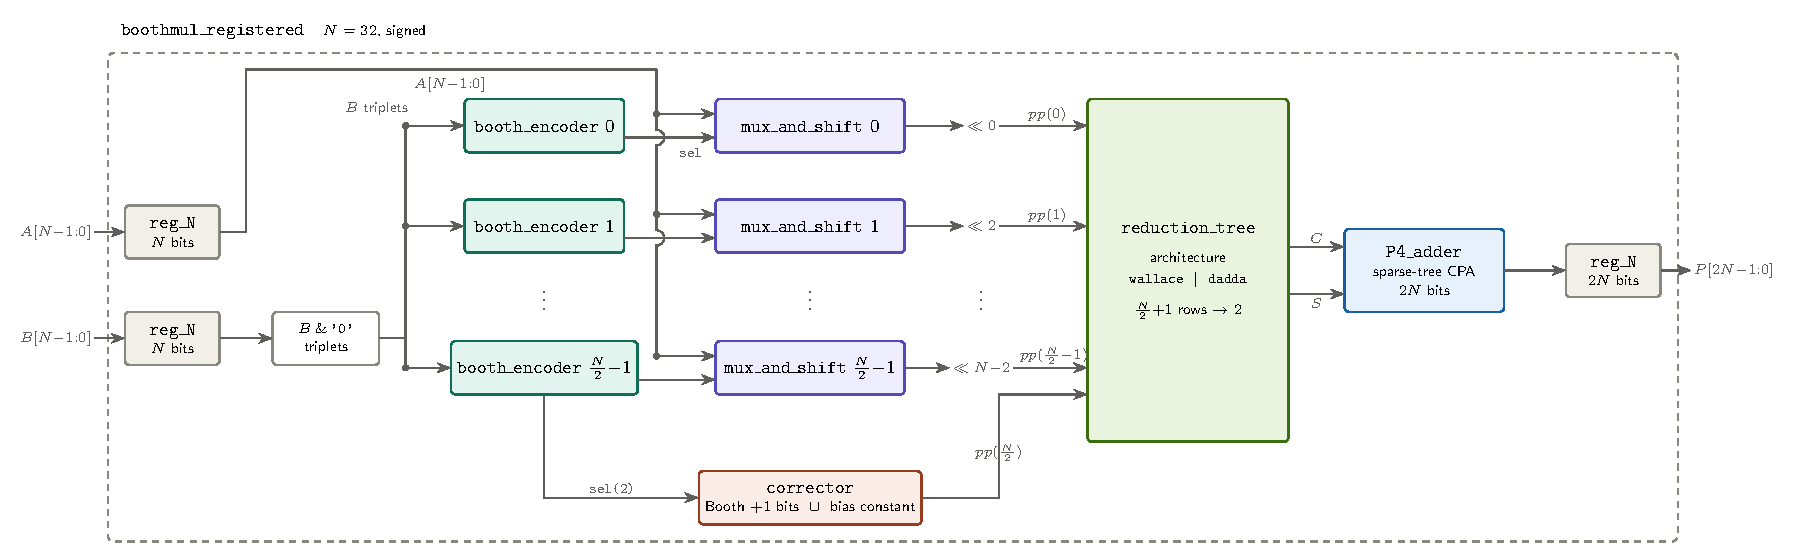
\includegraphics[width=\textwidth]{schematic.pdf}
\end{frame}

% =====================================================================
\begin{frame}{Radix-4 modified Booth recoding}

Overlapping triplets of $B$ --- bits $(2i{+}1,\,2i,\,2i{-}1)$, with $B_{-1}=0$
--- map to a signed digit $d_i\in\{0,\pm1,\pm2\}$:

\[
A \cdot B \;=\; \sum_{i=0}^{N/2-1} d_i \, A \cdot 4^{\,i}
\]

\begin{columns}[T]
\begin{column}{0.45\textwidth}
\centering\small
\begin{tabular}{@{}ccl@{}}
\toprule
triplet & $d_i$ & row \\
\midrule
000, 111 & $0$  & zeros \\
001, 010 & $+1$ & $+A$  \\
011      & $+2$ & $+2A$ \\
100      & $-2$ & $-2A$ \\
101, 110 & $-1$ & $-A$  \\
\bottomrule
\end{tabular}
\end{column}
\begin{column}{0.52\textwidth}
\small
$N/2$ rows instead of $N$. The reduction tree dominates area and delay, and its
cost grows with the row count, so halving the rows is the point of the recoding.

\vspace{6pt}
Multiplying by two is a wired shift and costs nothing.

\vspace{6pt}
{\color{accent}\textbf{Negation is not free.}} It is the origin of two of the
three optimizations.
\end{column}
\end{columns}

\end{frame}

% =====================================================================
\section{Optimization 1}

\begin{frame}{Optimization 1 --- the cost of the sign extension}

Row $i$ holds $m_i = d_i A$, which fits in $N+1$ bits of two's complement. Placed
at weight $2^{2i}$ in a $2N$-bit array and summed as an unsigned quantity, bit
$N$ must be replicated up to position $2N-1$.

\vspace{4pt}
Replicated bits in row $i$: $N-1-2i$. Across the array:

\[
\sum_{i=0}^{N/2-1} (N-1-2i)
\;=\;\frac{N}{2}(N-1)-\frac{N}{2}\Bigl(\frac{N}{2}-1\Bigr)
\;=\;\boxed{\frac{N^2}{4}}
\]

\vspace{4pt}
\centering\small
\begin{tabular}{@{}lrrr@{}}
\toprule
$N$ & total array bits & sign bits & fraction \\
\midrule
 8 &   56 &  16 & 28.6\% \\
16 &  208 &  64 & 30.8\% \\
32 &  800 & 256 & 32.0\% \\
\bottomrule
\end{tabular}

\vspace{4pt}
\raggedright\small
At $N=32$: $256$ of $800$ partial-product bits carry no information beyond the
single bit they replicate. Each must still be generated, routed and compressed.

\end{frame}

% =====================================================================
\begin{frame}{Optimization 1 --- the inversion identity}

For a two's complement number with sign bit $s$:
\[
m_i \;=\; -s\cdot 2^N + \sum_{j=0}^{N-1} m_{i,j}\,2^{\,j}
\]

Since $s+\bar{s}=1$ for a single bit, $-s = \bar{s}-1$, hence
\[
-s\cdot 2^N \;=\; \bar{s}\cdot 2^N - 2^N
\]

Define the \emph{stored} row --- low $N$ bits unchanged, sign bit inverted,
zeros above:
\[
R_i \;=\; \bar{s}\cdot 2^N + \sum_{j=0}^{N-1} m_{i,j}\,2^{\,j}
\qquad\Longrightarrow\qquad
\boxed{\,m_i \;=\; R_i - 2^N\,}
\]

\vspace{2pt}
The sign extension becomes one inverted bit. What remains is a constant error of
exactly $2^N$ per row --- independent of $A$, of the Booth digit, and of the row
index. Not an approximation.

\end{frame}

% =====================================================================
\begin{frame}{Optimization 1 --- the correction constant}

Summing the per-row bias over the array:
\[
E \;=\; \sum_{i=0}^{N/2-1} 2^{\,N+2i}
     \;=\; 2^N\cdot\frac{4^{N/2}-1}{3}
     \;=\; \frac{2^N(2^N-1)}{3}
\]

The datapath computes in $\mathbb{Z}/2^{2N}\mathbb{Z}$, so the correction is
simply the additive inverse:
\[
C \;=\; 2^{2N}-\frac{2^N(2^N-1)}{3}
   \;=\; 2^N\!\left(2^N-\frac{2^N-1}{3}\right)
\]

\begin{columns}[T]
\begin{column}{0.42\textwidth}
\centering\small
\begin{tabular}{@{}rl@{}}
\toprule
$N$ & $C$, bits $2N{-}1$ down to $N$ \\
\midrule
 4 & \texttt{0xB} \\
 8 & \texttt{0xAB} \\
16 & \texttt{0xAAAB} \\
32 & \texttt{0xAAAAAAAB} \\
\bottomrule
\end{tabular}
\end{column}
\begin{column}{0.55\textwidth}
\small
$C$ is a multiple of $2^N$: its lower $N$ bits are zero.

\vspace{4pt}
For even $N$, $(2^N-1)/3 = 0101\ldots01$, so $2^N$ minus it gives
$1010\ldots1011$. The repeating pattern comes from the factor $1/3$.
\end{column}
\end{columns}

\end{frame}

% =====================================================================
\begin{frame}[fragile]{Optimization 1 --- why it costs no extra row}

Booth already needs one extra row for the $+1$ that each one's-complement
negation owes. That row occupies \textbf{even positions of the lower half} only.
The constant $C$ occupies the \textbf{upper half} only. They share one row
without collision.

\begin{lstlisting}[style=vhdl]
architecture no_sign_extend of corrector is
  constant SE_CONST : std_logic_vector(2*N-1 downto 0) := sign_ext_const(N);
begin
  gen_neg: for i in 0 to N/2-1 generate      -- low half: Booth increments
    correction_v(2*i)   <= neg_bits(i);
    correction_v(2*i+1) <= '0';
  end generate;
  correction_v(2*N-1 downto N) <= SE_CONST(2*N-1 downto N);  -- high half
end architecture;
\end{lstlisting}

\small
The high half is a tie to the supply rails: no logic at all. $C$ is a $2N$-bit
quantity, too large for the VHDL integer type at $N=32$, so
\texttt{sign\_ext\_const} builds the pattern bit by bit at elaboration time.

\end{frame}

% =====================================================================
\begin{frame}{Optimization 1 --- measured}

\centering\small
\begin{tabular}{@{}lrrr@{}}
\toprule
& \textbf{baseline} & \textbf{optimized} & \textbf{change} \\
\midrule
Partial-product bits     & 800  & 561  & $-29.9\%$ \\
Total cells @ 3.0\,ns    & 4639 & 4455 & $-4.0\%$ \\
XOR $+$ XNOR @ 3.0\,ns   & 1346 & 1332 & $-1.0\%$ \\
Area @ 3.0\,ns           & 6501\um & 6196\um & $-4.7\%$ \\
Minimum area             & 6346\um & 5975\um & $-5.8\%$ \\
Minimum achieved period  & 1.86\,ns & 1.87\,ns & $+0.5\%$ \\
\bottomrule
\end{tabular}

\vspace{10pt}
\raggedright\small
\textbf{$29.9\%$ fewer bits, $5.8\%$ less area.} The removed bits are
constant-valued sign replications, and constant propagation already eliminates
most of the logic that would process them.

\vspace{4pt}
What the optimization removes with certainty --- and what constant propagation
cannot remove --- is the \emph{structural height of the columns}. That is what
Optimization~2 exploits.

\end{frame}

% =====================================================================
\section{Optimization 2}

\begin{frame}{Optimization 2 --- columns, dots, and an exact invariant}

The array is $2N$ columns; column $k$ holds $n_k$ \emph{dots} of weight $2^k$.
Reduce until no column has more than two.

\vspace{6pt}
\begin{columns}[T]
\begin{column}{0.48\textwidth}
\centering\small
\begin{tabular}{@{}lccc@{}}
\toprule
& \textbf{in} & \textbf{out} & \textbf{net dots} \\
\midrule
Full adder & 3 & 1 sum $+$ 1 carry & $-1$ \\
Half adder & 2 & 1 sum $+$ 1 carry & $0$ \\
\bottomrule
\end{tabular}
\end{column}
\begin{column}{0.48\textwidth}
\small
A half adder costs cells and reduces nothing. Minimising half adders is the
whole point of Dadda.
\end{column}
\end{columns}

\vspace{10pt}
This gives an exact invariant, independent of the schedule:
\[
\#\text{FA} \;=\; D_{\text{initial}} - D_{\text{final}}
\]

\vspace{2pt}
\small
At $N=32$: $561 - 126 = 435$. The schedule produces exactly $435$ --- used as
the correctness check on the whole algorithm.

\end{frame}

% =====================================================================
\begin{frame}[fragile]{Optimization 2 --- Wallace and Dadda}

\begin{columns}[T]
\begin{column}{0.48\textwidth}
\textbf{Wallace:} compress as early as possible. Every group of three dots gets
a full adder, at every stage.
\end{column}
\begin{column}{0.48\textwidth}
\textbf{Dadda:} compress as late as possible. Fix a target height per stage,
place only enough compressors to reach it.
\end{column}
\end{columns}

\vspace{8pt}
\[
d_0 = 2,\qquad d_{j+1}=\left\lfloor\tfrac{3}{2}d_j\right\rfloor
\;\Longrightarrow\; 2,\,3,\,4,\,6,\,9,\,13,\,19,\,28,\ldots
\]

$d_j$ is the largest height reducible to two in $j$ stages. At $N=32$ the array
has $17$ rows, $d_6=19\geq17$, so \textbf{six stages}: $17\to13\to9\to6\to4\to3\to2$.

\begin{lstlisting}[style=vhdl]
function height_dadda(lev : natural) return natural is
  variable temp : integer := 2;
begin
  for i in 0 to lev-1 loop temp := (temp*3)/2; end loop;
  return temp;
end function;
\end{lstlisting}

\end{frame}

% =====================================================================
\begin{frame}[fragile]{Optimization 2 --- the schedule is computed, not written}

The schedule depends only on the \emph{geometry} of the array, so it can be
computed before any signal exists. \texttt{constructing\_dadda} returns three
matrices indexed by (layer, row slot, column):

\vspace{2pt}
\centering\small
\begin{tabular}{@{}ll@{}}
\toprule
\texttt{FA\_matrix} & the three source slots of every full adder \\
\texttt{HA\_matrix} & the two source slots of every half adder \\
\texttt{remaining\_system} & the dots no compressor consumed \\
\bottomrule
\end{tabular}

\vspace{6pt}
\raggedright
Produced in one pass, kept consistent by mark-and-clear:

\begin{lstlisting}[style=vhdl]
while node_cnt < 3 loop
  if system(lev)(roww)(col) = '1' then
    node_cnt := node_cnt + 1;
    FA_matrix(lev)(roww)(col) := '1';   -- record the source slot
    system(lev)(roww)(col)    := '0';   -- and consume it
  end if;
  roww := roww + 1;
end loop;
\end{lstlisting}

\small
A consumed dot cannot be assigned twice, and cannot survive into the passed set.

\end{frame}

% =====================================================================
\begin{frame}[fragile]{Optimization 2 --- the carry accounting}

\small
The target height applies to the \emph{next} layer. Column $k$ of layer
$\mathrm{lev}-1$ receives (i) $C_{\mathrm{in}}$ carries from column $k-1$ of the
\textbf{same} stage, (ii) one sum bit per compressor, (iii) the dots no
compressor consumed:

\normalsize
\[
C_{\mathrm{in}} + (F+H) + (n-3F-2H) \;=\; C_{\mathrm{in}} + n - 2F - H
\;\;\leq\;\; d_{\mathrm{lev}-1}
\]

\small
A column must be sized against a quantity that \textbf{does not exist in its own
layer}. Omit $C_{\mathrm{in}}$ and the schedule is locally plausible and
globally wrong: columns overflow and the array never reaches two rows.

\begin{lstlisting}[style=vhdl]
count_temp := count + C_out_count;     -- own dots plus carries from col-1
while (count_temp > max_height) loop
  if    count_temp >= (max_height + 2) then count_temp := count_temp - 2; fa_id := fa_id + 1;
  elsif count_temp  = (max_height + 1) then ha_flag := 1; count_temp := count_temp - 1;
  end if;
end loop;
\end{lstlisting}

\end{frame}

% =====================================================================
\begin{frame}[fragile]{Optimization 2 --- recovering the port-map positions}

Slot order in column $k$ of the next layer is fixed:
carries from $k-1$, then sums, then passed dots.

\vspace{4pt}
\textbf{The problem:} a \texttt{generate} statement has no sequential state. Each
instance elaborates independently and cannot inherit a running counter from the
previous column. Every offset must be recomputable from the matrices alone.

\vspace{4pt}
\centering\scriptsize
\begin{tabular}{@{}ll@{}}
\toprule
\texttt{fa\_count\_col\_dadda} & full adders in a column \\
\texttt{ha\_flag\_col\_dadda} & $1$ if the column has a half adder \\
\texttt{num\_C\_out\_from\_prev\_col} & $C_{\mathrm{in}}$, \textbf{recomputed} by counting column $k-1$ \\
\texttt{fa\_arg\_func} / \texttt{ha\_arg\_func} & source row indices of each compressor \\
\texttt{remaining\_counting\_func} / \texttt{remaining\_bit\_pos} & the passed dots and their rows \\
\bottomrule
\end{tabular}

\vspace{4pt}
\raggedright
\begin{lstlisting}[style=vhdl]
FA_i : FA port map (
  A  => layer(lev)(FA_args(ID)(0))(col),
  B  => layer(lev)(FA_args(ID)(1))(col),
  Ci => layer(lev)(FA_args(ID)(2))(col),
  S  => layer(lev-1)(ID + C_out_counting)(col),
  Co => layer(lev-1)(ID)(col+1));
\end{lstlisting}

\end{frame}

% =====================================================================
\begin{frame}{Optimization 2 --- the schedule is generic in $N$}

\centering\small
\begin{tabular}{@{}rrrrrrrrr@{}}
\toprule
& & \multicolumn{2}{c}{\textbf{array dots}} & \multicolumn{4}{c}{\textbf{Dadda}} & \textbf{Wallace} \\
\cmidrule(lr){3-4}\cmidrule(lr){5-8}\cmidrule(lr){9-9}
$N$ & rows & baseline & optimized & stages & FA & HA & cells & FA instances \\
\midrule
 8 &  5 &   56 &   45 & 3 &   15 &  9 &   24 &   48 \\
16 &  9 &  208 &  153 & 4 &   91 & 21 &  112 &  224 \\
\textbf{32} & \textbf{17} & \textbf{800} & \textbf{561} & \textbf{6} & \textbf{435} & \textbf{45} & \textbf{480} & \textbf{960} \\
64 & 33 & 3136 & 2145 & 8 & 1891 & 93 & 1984 & 3968 \\
\bottomrule
\end{tabular}

\vspace{8pt}
\raggedright\small
Per-stage at $N=32$: $28/92/111/94/53/57$ full adders and $12/12/9/6/3/3$ half
adders.

\vspace{6pt}
The Wallace implementation instantiates carry-save adders at the full $2N$
width: $960$ full adder instances against $435$ FA $+$ $45$ HA. Many Wallace
instances have constant inputs and are removed by the tool --- but constant
propagation cannot recover the shorter critical path a column-scheduled tree
provides.

\end{frame}

% =====================================================================
\begin{frame}{Optimization 2 --- measured}

\centering\small
\begin{tabular}{@{}lrrr@{}}
\toprule
& \textbf{Wallace} & \textbf{Dadda} & \textbf{change} \\
\midrule
Adder cells in the RTL   & 960 FA & 435 FA $+$ 45 HA & $-50\%$ \\
Total cells @ 3.0\,ns    & 4455 & 3936 & $-11.7\%$ \\
Area @ 3.0\,ns           & 6196\um & 5725\um & $-7.6\%$ \\
Minimum area             & 5975\um & 5620\um & $-5.9\%$ \\
\textbf{Min. achieved period} & \textbf{1.87\,ns} & \textbf{1.78\,ns} & $\mathbf{-4.8\%}$ \\
\bottomrule
\end{tabular}

\vspace{10pt}
\raggedright\small
The largest single improvement in \textbf{delay} of the three optimizations ---
which is what a shorter, more uniform reduction depth should produce.

\end{frame}

% =====================================================================
\section{Optimization 3}

\begin{frame}{Optimization 3 --- the diagnosis}

After Optimization~2 the design was still $1180$\um{} larger than the inferred
reference. A cell census localised the difference.

\vspace{4pt}
\centering\small
\begin{tabular}{@{}lrrrr@{}}
\toprule
@ 3.0\,ns & \textbf{XOR $+$ XNOR} & \textbf{FA cells} & \textbf{INV} & \textbf{total} \\
\midrule
Structural, Dadda       & 1230 & 117 & 505 & 3936 \\
Inferred \texttt{A * B} &  559 & 268 & 311 & 3035 \\
\bottomrule
\end{tabular}

\vspace{8pt}
\raggedright\small
\textbf{$671$ excess XOR cells, and only $117$ of $435$ scheduled full adders
mapped to library adder cells.} One cause for both:

\vspace{4pt}
\texttt{mux\_and\_shift} builds a row in two steps --- a multiplexer picks
$A$, $2A$ or zero, then every bit is XORed with $\mathtt{sel}(2)$ to negate.
That is $N+1$ XOR2 per row $\times$ $16$ rows $= 528$ cells $\approx 843$\um{}
doing nothing but conditional inversion.

\vspace{4pt}
A full adder is itself XOR-dominated. With an XOR layer feeding the tree, the
mapper sees cones that mix negation and compression, and decomposes them into
generic gates instead of recognising \texttt{FA\_X1}. The low adder count is a
\emph{symptom}, not a separate problem.

\end{frame}

% =====================================================================
\begin{frame}{Optimization 3 --- merging selection and negation}

Two sources, decoded once per row into four mutually exclusive conditions:

\[
\mathrm{src}_1 = A_{N-1}\Vert A \;(\pm A), \qquad
\mathrm{src}_2 = A \Vert \mathtt{'0'} \;(\pm 2A)
\]
\[
\begin{aligned}
c_{+1} &= \mathtt{sel}(0)\overline{\mathtt{sel}(1)}\,\overline{\mathtt{sel}(2)}, &
c_{-1} &= \mathtt{sel}(0)\overline{\mathtt{sel}(1)}\,\mathtt{sel}(2), \\
c_{+2} &= \mathtt{sel}(0)\mathtt{sel}(1)\overline{\mathtt{sel}(2)}, &
c_{-2} &= \mathtt{sel}(0)\mathtt{sel}(1)\mathtt{sel}(2).
\end{aligned}
\]

\[
\boxed{\;q_i = c_{+1}\mathrm{src}_{1,i} + c_{-1}\overline{\mathrm{src}_{1,i}}
            + c_{+2}\mathrm{src}_{2,i} + c_{-2}\overline{\mathrm{src}_{2,i}}\;}
\]

\small
\textbf{Four terms suffice.} The zero row is covered implicitly: all four
conditions are false when $\mathtt{sel}(0)=0$. This is complete provided the
encoder never requests a \emph{negated zero} --- and the only codes with
$\mathtt{sel}(2)=1$ are $101$ and $111$, both of which have $\mathtt{sel}(0)=1$.
The property follows from the encoding table; it is not an assumption on it.

\vspace{4pt}
Two-level sum of products over four literals $\rightarrow$ one AOI/OAI compound
cell per bit. No XOR anywhere. $\overline{\mathrm{src}_1},
\overline{\mathrm{src}_2}$ are the same function of $A$ in all $16$ rows, so one
set of inverters is shared.

\end{frame}

% =====================================================================
\begin{frame}{Optimization 3 --- measured}

\centering\small
\begin{tabular}{@{}lrrrrr@{}}
\toprule
@ 3.0\,ns & \textbf{XOR $+$ XNOR} & \textbf{FA cells} & \textbf{AOI/OAI} & \textbf{total} & \textbf{area} \\
\midrule
Dadda, separate negation & 1230 & 117 & 1405 & 3936 & 5725\um \\
\textbf{Dadda, fused selector} & \textbf{85} & \textbf{448} & 1311 & \textbf{2819} & \textbf{5125\um} \\
Inferred \texttt{A * B}  &  559 & 268 &  950 & 3035 & 4910\um \\
\bottomrule
\end{tabular}

\vspace{8pt}
\centering\small
\begin{tabular}{@{}lrrr@{}}
\toprule
& \textbf{before} & \textbf{after} & \textbf{change} \\
\midrule
Minimum area            & 5620\um & 5029\um & $-10.5\%$ \\
Minimum achieved period & 1.78\,ns & 1.76\,ns & $-1.1\%$ \\
\bottomrule
\end{tabular}

\vspace{8pt}
\raggedright\small
XOR cells $1230 \rightarrow 85$. Adder cells $117 \rightarrow 448$ --- within
$7\%$ of the $480$ compressors the Dadda schedule actually contains.

\vspace{4pt}
\textbf{The gain is indirect.} Removing the XOR layer did not just delete $528$
cells; it let the mapper recognise the compressors that had been in the RTL all
along.

\end{frame}

% =====================================================================
\begin{frame}{Verification}

\begin{columns}[T]
\begin{column}{0.48\textwidth}
One self-checking testbench for all variants, reading \texttt{NBIT} from
\texttt{common\_pkg}:

\vspace{4pt}
\centering\small
\begin{tabular}{@{}ll@{}}
\toprule
\texttt{NBIT} & coverage \\
\midrule
$\leq 8$ & exhaustive, $65\,536$ pairs \\
$> 8$    & corners $+$ $20\,000$ random \\
\bottomrule
\end{tabular}

\vspace{6pt}
\raggedright\small
Reference model: \texttt{signed(A) * signed(B)} truncated to $2N$ bits.
Mismatches are counted, not asserted, so a failing variant reports how badly it
fails.
\end{column}

\begin{column}{0.48\textwidth}
\small
Exhaustive coverage at $N=8$ is worth more than random coverage at $N=32$: the
properties under test --- the recoding table, the bias cancellation, the
four-term cover, the column schedule --- are structural, and fail identically at
both widths.

\vspace{6pt}
\textbf{Two defects found this way:}

\vspace{2pt}
$-2A$ formed by shifting without complementing: $256$ of $1280$ directed cases
failed.

\vspace{2pt}
A variant missing the Booth increment entirely: $61\,440$ of $65\,536$ failed.
Its \emph{area} results looked excellent, because the missing logic was
genuinely absent.
\end{column}
\end{columns}

\end{frame}

% =====================================================================
\begin{frame}{Synthesis methodology}

\begin{columns}[T]
\begin{column}{0.46\textwidth}
\centering\scriptsize
\begin{tabular}{@{}ll@{}}
\toprule
Library & Nangate 45\,nm, typical ECSM \\
Tool    & DC W-2024.09-SP2, \texttt{compile\_ultra} \\
Wire load & \texttt{5K\_hvratio\_1\_4} \\
Uncertainty & $0.05$\,ns \\
Input / output delay & $0.25$ / $0.15$\,ns, \textbf{absolute} \\
Driving cell & \texttt{BUF\_X4}, load $0.05$\,pF \\
Max transition & $0.20$\,ns \\
Sweep & $21$ periods, $1.0$ to $6.0$\,ns \\
\bottomrule
\end{tabular}
\end{column}

\begin{column}{0.50\textwidth}
\footnotesize
\textbf{Achieved period, not constraint.}
\[
T_{\text{achieved}} = T_{\text{constraint}} - \text{slack}
\]
A violated run still gives a valid netlist, just a slower one. Discarding those
would discard the fastest netlists, since the tool only builds aggressive
structures under a tight constraint. The identity is exact only because the port
delays are absolute rather than a fraction of the period.

\vspace{6pt}
\textbf{\texttt{compile\_ultra} is not monotonic.} A looser period can give a
larger netlist. Verified not to be the area constraint: a controlled run without
\texttt{set\_max\_area} gave identical minimum periods and $<3\%$ area
difference, still non-monotonic. All curves are therefore Pareto fronts over the
whole sweep.
\end{column}
\end{columns}

\end{frame}

% =====================================================================
\section{Results}

\begin{frame}{Results --- summary}

\centering\small
\begin{tabular}{@{}lrrrr@{}}
\toprule
\textbf{Variant} & \textbf{min. achieved} & \textbf{min. area} & \textbf{cells @ 3.0\,ns} & \textbf{gap closed} \\
\midrule
Wallace, sign-extended (baseline)    & 1.86\,ns & 6346\um & 4639 & --- \\
\quad $+$ sign-extension elimination & 1.87\,ns & 5975\um & 4455 & 19.5\% \\
\quad $+$ Dadda reduction            & 1.78\,ns & 5620\um & 3936 & 38.1\% \\
\quad \textbf{$+$ fused selector}    & \textbf{1.76\,ns} & \textbf{5029\um} & \textbf{2819} & \textbf{69.1\%} \\
\midrule
Behavioural Booth (adder chain)      & 2.01\,ns & 6210\um & 4863 & 7.1\% \\
Inferred \texttt{A * B}              & 1.63\,ns & 4441\um & 3035 & reference \\
\bottomrule
\end{tabular}

\vspace{10pt}
\raggedright\small
Area gap to the reference closed by $69.1\%$; delay gap reduced from $0.23$\,ns
to $0.13$\,ns.

\vspace{4pt}
The behavioural variant --- a chain of signed additions instead of a tree --- is
the slowest design in the sweep, but not the largest: the tool builds its own
carry-save structures rather than using the instantiated ones. Its \emph{timing}
is the informative figure.

\end{frame}

% =====================================================================
\begin{frame}{Results --- the Pareto front}
\centering
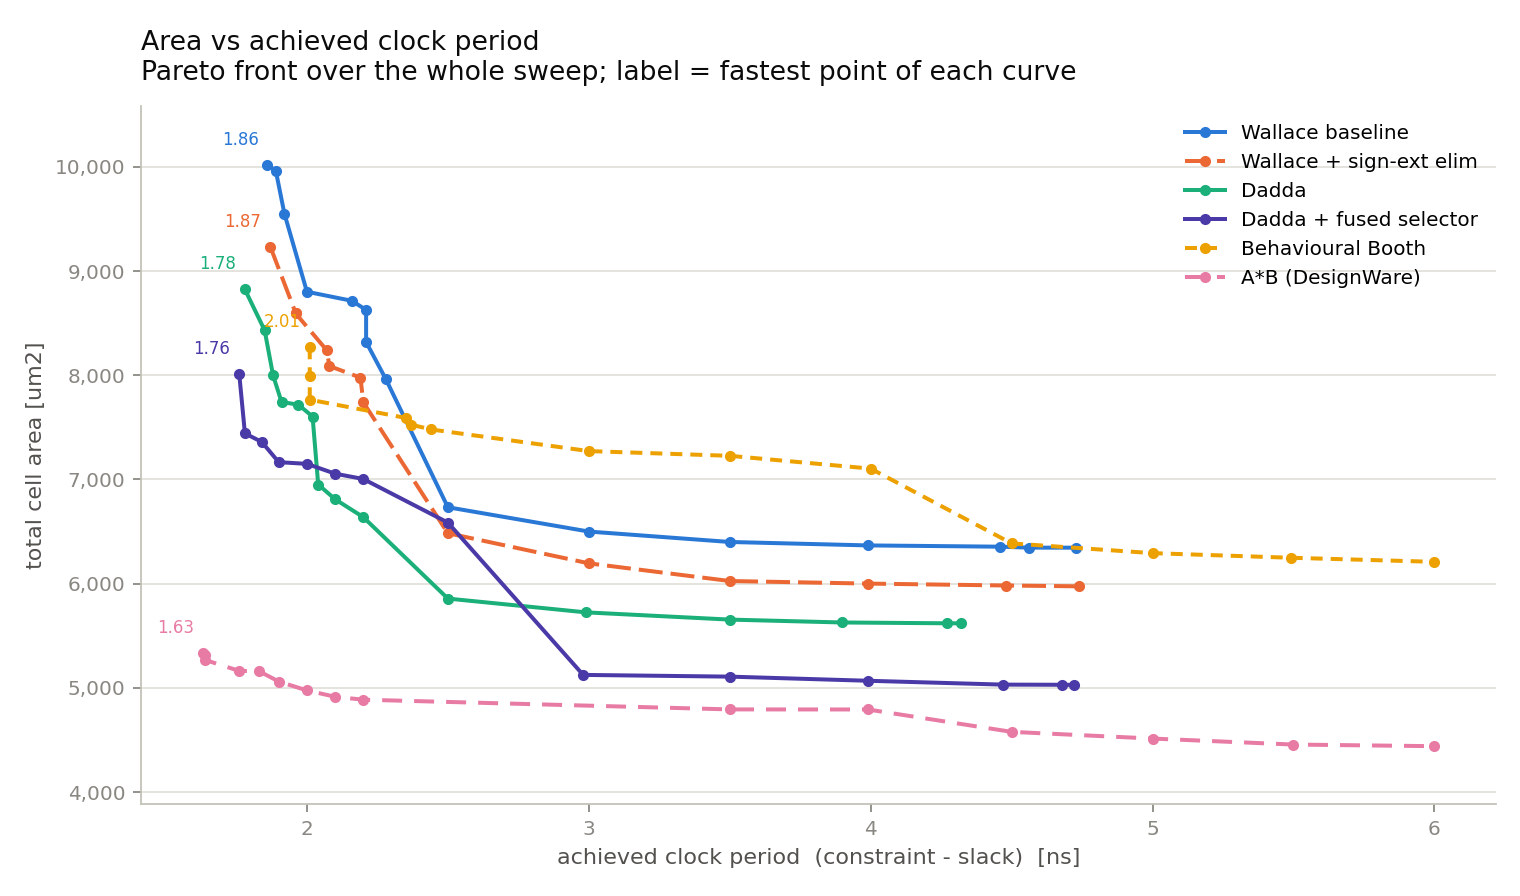
\includegraphics[width=0.78\textwidth]{figures/pareto_area_vs_achieved_main.png}

\vspace{-2pt}
\footnotesize
Each curve is the Pareto front of one variant over all $21$ runs; dominated
points omitted. The ordering holds across the whole range, and the separation is
widest at relaxed timing.
\end{frame}

% =====================================================================
\begin{frame}{Results --- a genuine crossing}
\begin{columns}[T]
\begin{column}{0.58\textwidth}
\centering
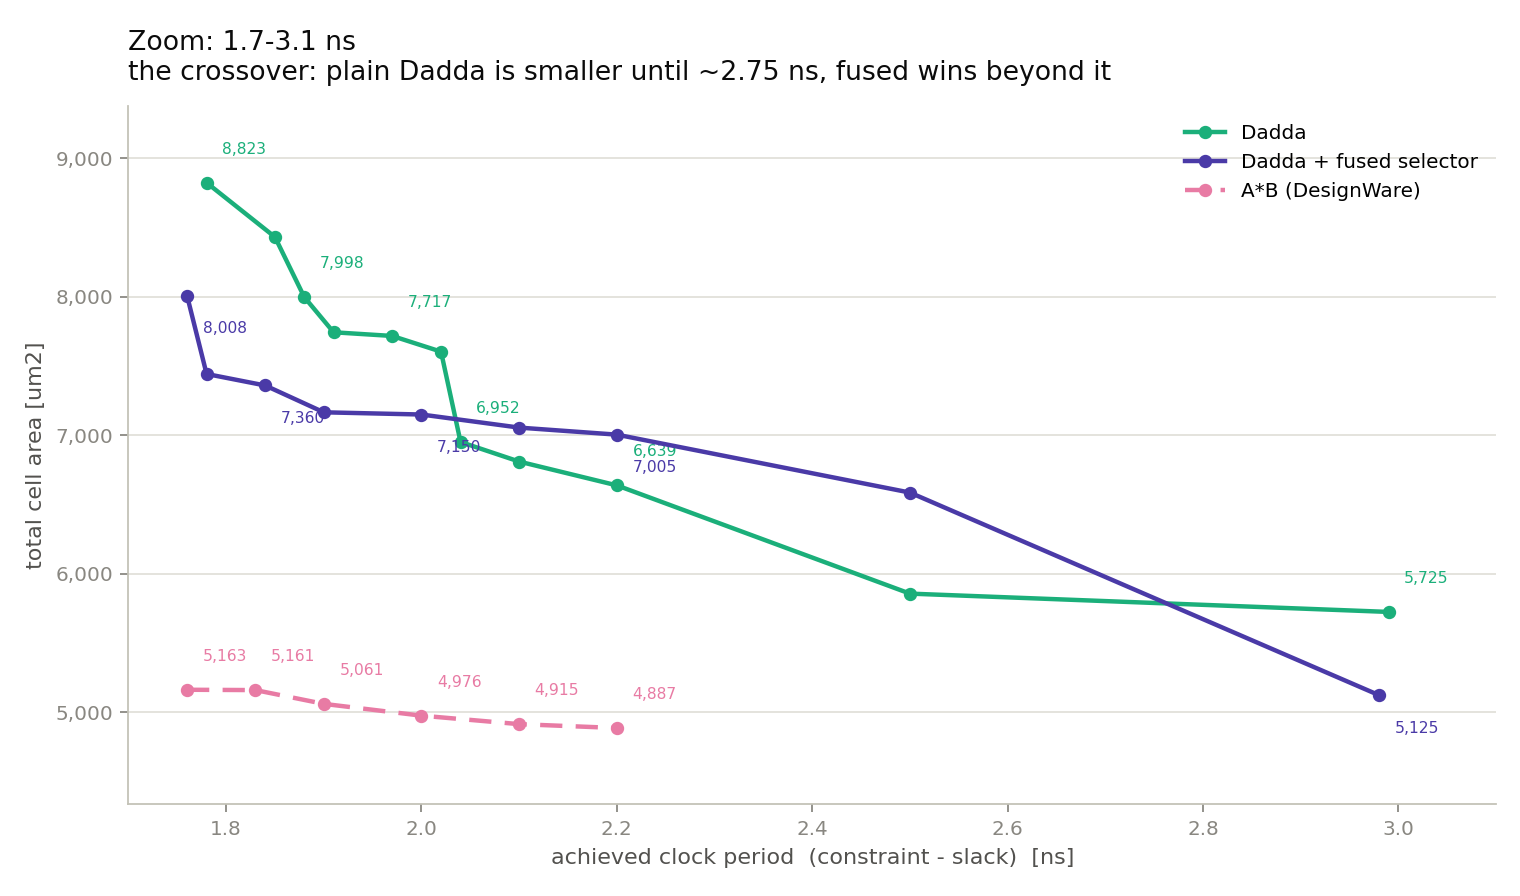
\includegraphics[width=\textwidth]{figures/pareto_zoom_main.png}
\end{column}
\begin{column}{0.40\textwidth}
\footnotesize
The two Dadda variants cross \textbf{twice}. Near $2.0$\,ns the variant with
separate negation is the smaller of the two.

\vspace{5pt}
The fused selector presents deeper compound gates. At intermediate constraints
the tool must upsize them to meet timing, and the upsizing costs more than the
XOR cells that were removed.

\vspace{5pt}
At relaxed timing the upsizing is unnecessary and the fused variant is
$591$\um{} smaller; at tight timing it is faster.

\vspace{5pt}
Reproduced across adjacent constraint points, and visible in the census as a
shift in \emph{drive strengths} rather than cell counts: an architectural
trade-off, not optimizer noise.
\end{column}
\end{columns}
\end{frame}

% =====================================================================
\begin{frame}{Conclusions}

\begin{columns}[T]
\begin{column}{0.52\textwidth}
\small
\textbf{Result.} $1.76$\,ns and $5029$\um{} against $1.63$\,ns and $4441$\um{}
for an inferred \texttt{A * B} multiplier. $69.1\%$ of the initial area gap
recovered.

\vspace{6pt}
\textbf{The contributions were unequal, and not as predicted.}

\vspace{2pt}
Sign-extension elimination removes $29.9\%$ of the array but $5.8\%$ of the
area --- constant propagation had already taken most of it.

\vspace{2pt}
The Dadda schedule gives a comparable area gain and the largest delay gain.

\vspace{2pt}
The fused selector gives the largest area gain, indirectly: not the $528$ XOR
cells it deletes, but the $331$ additional full adders the mapper can then
recognise.
\end{column}

\begin{column}{0.44\textwidth}
\small
\textbf{The general point.}\\[2pt]
The cost of an RTL construct is set as much by what it prevents the tool from
recognising as by the gates it implies. One layer of XOR gates between the row
generators and the tree was worth $\approx 600$\um{} --- by concealing the
structure behind it.

\vspace{10pt}
\textbf{Open.}
\begin{itemize}\itemsep1pt\small
\item Switching activity and power
\item Gate-level simulation against SDF
\item Sweep below $1.0$\,ns
\item Baugh--Wooley comparison
\end{itemize}
\end{column}
\end{columns}

\end{frame}

\end{document}
